\documentclass[runningheads]{llncs}

\usepackage{geometry}
\geometry{
  a4paper,         % or letterpaper
  textwidth=15cm,  % llncs has 12.2cm
  textheight=24cm, % llncs has 19.3cm
  heightrounded,   % integer number of lines
  hratio=1:1,      % horizontally centered
  vratio=2:3,      % not vertically centered
}


\usepackage[T1]{fontenc}
\usepackage[utf8]{inputenc}	%Umlaute
\usepackage{amssymb, amsmath}
\usepackage[ngerman]{babel}
\usepackage{graphicx, subcaption}
\usepackage{hyperref}
\usepackage{biblatex}

\captionsetup[table]{skip=10pt}
\addbibresource{sources.bib}

\begin{document}

\title{Kolorierung von Nah-Infrarotbildern}
\subtitle{Exposé Projektgruppe Intelligente Sehsysteme}
\author{Ayk Borstelmann}
\authorrunning{A. Borstelmann}
\institute{Institut für Informatik, Friedrich-Hirzebruch-Allee 8, 53115 Bonn
\email{ayk.borstelmann@uni-bonn.de}
}
\maketitle
%
%
%
\section{Zielsetzung}
Typischerweise werden Kameras für Wild- und Überwachungsszenarien als Sensoren benutzt.
Im Gegensatz zu normalen RGB Kameras haben jedoch Infrarotbilder (NIR-Bilder) einige Vorteile. 
So kann auch ohne zusätzliche Lichtquellen, welche bspw. das Wild blenden oder gar verschrecken, 
das für die Augen von Mensch und Wild unsichtbaren Licht des Infrarotspektrums für detaillierte Nachtaufnahmen sorgen. 
Für Menschen sind NIR Bilder jedoch schwierig zu interpretieren, da diese nur in schwarz-weiß darstellbar sind und 
somit die für die menschliche Interpretation hilfreiche Farbunterscheidung der Szenen fehlt. 
Auch in Objekterkennung kann es von Vorteil seien Farbbilder zur Verfügung zu haben.

Innerhalb dieser Projektarbeit soll vergleichend Ansätze, welche Infrarotbilder - insbesondere Wildtieraufnahmen - zuverlässig koloriert, implementiert und evaluiert werden. 

Da NIR-Bilder in Schwarz-Weiß Format vorliegen ist die Kolorierung eng verwandt mit der Kolorierung von Schwarz-Weiß-Bildern aus dem sichtbaren Spektrum.
Allerdings sind Methoden zum Kolorieren von Schwarz-Weiß-Bildern nicht ideal für Kolorierung von NIR-Bildern. 
Schwarz-Weiß-Bilder lassen sich als Beleuchtung der Szene und somit Intensität des RGB Pixels interpretieren, womit nur noch die entsprechenden Farbwerte zu schätzen sind. 
Infrarotbildern sind jedoch nicht als Beleuchtung der Szene geeignet, da sich der Reflexionsgrad von Infrarotlicht von sichtbarem Licht unterscheidet. 
Auch der Anwendungskontext von Wildtieraufnahmen bringt zusätzliche Herausforderungen. 
Insbesondere nachtaktive Tiere werden in schlechten Lichtsituationen aufgenommen und liegen somit häufig nur in Infrarot vor, ohne entsprechende kolorierte Gegenstücke.
Auch die Bewegung von Tieren und mögliche Verschiebung der beiden Kameras erschwert die Aufnahme von pixelgleichen NIR- und RGB Paaren, welche für manche Methoden vorausgesetzt werden.   

\section{Daten}
Als Datensatz für Training und Evaluation wird Caltech Camera Traps \cite*{caltech} benutzt. 
Dieser enthält 243,100 Bilder aus den Vereinigten Staaten und enthält insbesondere auch Infrarotbilder.
Innerhalb dieser Bilder sind 21 verschiedene Tiere vertreten und etwa 70 \% der Bilder sind als \glqq leer\grqq \ klassifiziert \cite*{caltech}.
Somit ist beim Auswählen für Trainingsdaten ein ausreichendes Auftreten von nicht leeren Bilder zu beachten.  
Typischerweise sind die Bilder in FullHD Auflösung gegeben und in Kameraserien eingeteilt. 
Für Methoden, welche gepaarte NIR- und RGB-Paare benötigen, kann somit anhand der Kameraserieneinteilung effizient nach Gegenstücken mit gleichen Winkel gesucht werden.  

\section{Methoden}
Um NIR-Bilder zu kolorieren, existieren bereits einige Ansätze. 

So stellte Limmer \textit{et. al.} eine auf Deep Convolutional Neural Networks (CNN) beruhende Methode vor, 
welche Paaren von pixelgleichen NIR- und RGB Bilder zum Training benötigt. Dabei wird zuerst in einem Preprocessingschritt eine normalisierte Bildpyramide
aus der NIR Eingabe aufgebaut, welche dann als Input für das CNN dient. Anschließend wird das ausgegebene Bild des Netzwerkes mit Details aus dem Inputbild bereichert.
Limmer \textit{et. al.} konnten die pixelgleichen NIR- und RGB Paare anhand eines Datensatzes erlangen, welcher mit einer speziellen multi-CCD Kamera aufgenommen wurde. \cite{limmer2016infrared}   

Ebenfalls pixelgleiche NIR- und RGB Bilder zum Training werden von Dong \textit{et. al.} für das Trainieren ihres Ansatzes benötigt. 
Dabei benutzt Dong \textit{et. al.} zwei Encoder-Decoder CNNs (\glqq S-Shape Network\grqq), ein Hauptnetzwerk, welches den RGB Wert schätzt (\glqq ColorNet\grqq) und ein zweites, 
welches während des Trainings das Erhalten von Details in Form einer Loss-Funktion forciert (\glqq EdgeNet\grqq). 
Um die Pixelgleichheit in ihrem Datensatz herzustellen, 
benutzten Dong \textit{et. al.} zuerst eine merkmalbasierte Methode, um die Übereinstimmung von Bildern zu erkennen 
und dann geometrische Transformationen, um die Gleichheit zu erzeugen.    
Trainiert wurde ihr Netzwerk auf 224 $\times$ 244 großen Bildern \cite{dong2018infrared}.

Der Ansatz \glqq CyclicGAN\grqq \ (Cyclic Generative Adversial Network) von Mehri \textit{et. al.} benötigt keine NIR- und RGB-Bildpaare.
Stattdessen werden zwei Encoder-Decoder Netzwerke benutzt, um sowohl NIR- in RGB-Bilder als auch RGB- in NIR Bilder zu transformieren (Generators).
Ein Klassifikationsnetzwerk (Discriminator) schätzt anschließend, ob das Bild ein echtes oder generiertes ist. Die beiden Netze optimieren sich gegenseitig.
Das gesamte Netzwerk kann sowohl RGB- als auch NIR-Bilder als Eingabe erhalten, für die keine entsprechenden Gegenstücke existieren \cite{mehri2019colorizing}.

Sowohl der CyclicGAN Ansatz von Mehri \textit{et. al.} als auch die S-Shape Methode von Dong \textit{et. al.} benutzten Encoder-Decoder Architekturen, 
welche sich an U-Net, insbesondere der Aufbau der Skip-Connections \cite{unet} orientieren und sind sich somit sehr ähnlich \cite{dong2018infrared,mehri2019colorizing}. 
Limmer \textit{et. al.} hingegen benutzten keine Skip-Connections in ihrem Netzwerk und setzten stattdessen auf Netzwerktiefe und kleine Filtergrößen \cite{limmer2016infrared} 

In dem Anwendungskontext der Wildtieraufnahmen könnte die fehlende Notwendigkeit von pixelgleichen NIR- und RGB-Bild Paaren als vorteilhaft herausstellen.
Somit ist der CyclicGAN Ansatz von Mehri \textit{et. al.} \cite*{mehri2019colorizing} möglicherweise am besten als Grundlage geeignet. 
Alternativ könnte sich die Methode von Dong \textit{et. al.}, um pixelgleiche Bildpaare zu erzeugen und dann ein entsprechendes S-Shape Netzwerk zu trainieren \cite*{dong2018infrared}, ebenfalls bewähren.  

\section{Zeitplanung}

Grundlegend lässt das Projekt in 5 Arbeitsschritte einteilen (\autoref{fig:planung}). Zuerst muss der Datensatz Caltech Camera Traps heruntergeladen und ein Ausschnitt davon in Trainings- und Testdaten eingeteilt werden. 
Dabei ist es wichtig, dass Trainings- und Testdaten ausreichend Tieraufnahmen enthalten, da der Datensatz etwa 70 \% als leer markierte Bilder enthält \cite{caltech}. Für diesen Schritt ist ein Zeitraum von 2 Wochen einkalkuliert. 
Anschließend kann Implementation, Testen und Optimieren von CyclicGAN von Mehri \textit{et. al.} \cite*{mehri2019colorizing} auf diesem Datensatz begonnen werden (ca. 4 Wochen). 
Vergleichend dazu soll danach der S-Shape Ansatz von Dong \textit{et. al.} \cite*{dong2018infrared} umgesetzt werden. 
Dazu zählt das Finden und Transformieren von Inputpaaren, sowie die Implementation, das Testen als auch das Optimieren der Methode auf Wildtieraufnahmen. Schätzungsweise benötigt dieser Arbeitsschritt ebenfalls 4 Wochen. 
Schlussendlich soll der jeweils bessere Ansatz weiter anhand aktueller Forschung verbessert oder gar ein alternativer Ansatz implementiert und abschließend evaluiert werden (\autoref{fig:planung}).  

\begin{figure}
    \centering
    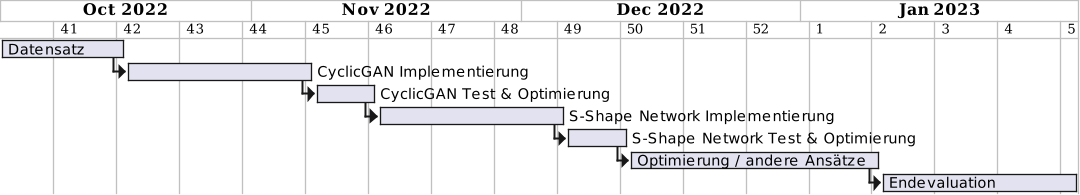
\includegraphics[width=\textwidth]{planung.png}
    \caption{
        Zeitplanung
    }
    \label{fig:planung}
\end{figure}

\printbibliography

\end{document}
